\subsection{Đề 04}
\Opensolutionfile{ans}[ans/ans-CTST-0-OTGK1-De04-LC]
\caulc
\begin{ex}%[1D1N1-9]
	Trong các câu sau, câu nào là mệnh đề?
	\choice
	{\True Phương trình $x^2-3x+1=0$ vô nghiệm}
	{Đề thi môn Toán khó quá!}
	{Không được làm việc riêng trong giờ học}
	{Bạn có đi học không?}
	\loigiai{
		Phương trình $x^2-3x+1=0$ vô nghiệm là mệnh đề.
	}
\end{ex}

\begin{ex}%[0D1N2-1]
	Hãy viết tập hợp sau bằng cách nêu tính chất đặc trưng cho các phần tử của tập hợp $A=\{0;4;8;12\}$.
	\choice
	{$A = \{ x \in \mathbb{R} \mid x \,\vdots\, 4 \text{và} x \le 14 \}$}
	{$A = \{ x \in \mathbb{Z} \mid x \,\vdots\, 4 \text{và} x \le 15 \}$}
	{\True $A = \{ x \in \mathbb{N} \mid x \,\vdots\, 4\text{và} x \le 15 \}$}
	{$A = \{ x \in \mathbb{N} \mid x \,\vdots\, 5 \text{và} x \le 15 \}$}
	\loigiai{
		Ta có $A=\{x\in \mathbb{N}\mid x \,\vdots\, 4 \text{và} x \le 15 \}$.
	}
\end{ex}
\begin{ex}%[0D1N2-1]
	Tập hợp $A=\{x\in \mathbb{R}\mid 4x+1>10 \}$ bằng tập hợp nào dưới đây?
	\choice
	{$\left(\dfrac{9}{4};+\infty\right)$}
	{$\left(- \dfrac{9}{4};+\infty\right)$}
	{$\left[\dfrac{9}{4};+\infty\right)$}
	{\True $\left(\dfrac{9}{4};+\infty\right)$}
	\loigiai{
		Ta có $4x+1>10 \Leftrightarrow x\in \left(\dfrac{9}{4};+\infty\right)$.\\
		Vậy $A=\left(\dfrac{9}{4};+\infty\right)$.
	}
\end{ex}
\begin{ex}%[0D1N3-1]
	Hình vẽ dưới là biểu diễn của tập hợp nào sau đây?
	\begin{center}
		\begin{tikzpicture}
			\def\a{-6}
			\def\b{5}
			\draw[-stealth] (\a-2,0)--(\b+2,0);
			\fill[pattern=north east lines]
			(\a,-.1) rectangle (\b,.1);
			%# (\a-2,-.1) rectangle (\a,.1)
			%# (\b,-.1) rectangle (\b+2,.1);
			\path
			(0,0) node{$|$} node[label=-90:$0$]{}
			(\a,0) node{$)$} node[label=-90:${-6}$]{}
			(\b,0) node{$[$} node[label=-90:${5}$]{};
	\end{tikzpicture}\end{center}
	\choice
	{$[-6;5)$}
	{\True $(-\infty;-6)\cup [5;+\infty)$}
	{$(-\infty;-6)\cup (5;+\infty)$}
	{$(-6;5]$}
	\loigiai{
		Hình vẽ biểu diễn tập hợp trục số trên là tập hợp $(-\infty;-6)\cup [5; +\infty)$.
	}
\end{ex}

\begin{ex}%[0D2N1-1]
	Bất phương trình nào sau đây là bất phương trình bậc nhất hai ẩn?
	\choice
	{\True $7x+3y\ge 6$}
	{$5y^3-3<7$}
	{$(7x-6y)(3x+7y)\le 7$}
	{$6x^2+2y^2<2$}
	\loigiai{
		Bất phương trình bậc nhất hai ẩn là $7x+3y\ge 6$
	}
\end{ex}

\begin{ex}%[0D2N2-2]
	Cặp số $(1; -3)$ là nghiệm của hệ bất phương trình nào sau đây?
	\choice
	{$\heva{&4x-y+4\le 0\\&x+y+6< 0}$}
	{\True $\heva{&x+y-6\le 0\\&4x+2y-8\le 0}$}
	{$\heva{&- x+5y-10>0\\&-5x+3y+7\ge 0}$}
	{$\heva{&5x+3y-2>0\\&5x+3y+3>0}$}
	\loigiai{
		Ta có hệ bất phương trình
		$$\heva{&x+y-6\le 0\\&4x+2y-8\le 0}$$
		Với $f_1(x,y)=x+y-6$, ta có $f_1(1,-3)=-8\le 0$.\\
		Với $f_2(x,y)=4x+2y-8$, ta có $f_2(1,-3)=-10\le 0$.\\
		Vậy cặp số $(1;-3)$ là nghiệm của hệ bất phương trình $\heva{&x+y-6\le 0 \\ &4x+2y-8\le 0}$.
	}
\end{ex}
\begin{ex}%[0D3N1-2]
	Tìm tập xác định của hàm số $y=\sqrt{-8x+5}$.
	\choice
	{$\mathscr{D}=(0; +\infty)$}
	{$\mathscr{D}=\mathbb{R}$}
	{$\mathscr{D}=(-\infty;0)$}
	{\True $\mathscr{D}=\Big(-\infty;\dfrac{5}{8}\Big]$}
	\loigiai{
		Hàm số $y=\sqrt{-8x+5}$ xác định khi $-8x+5\ge 0\Leftrightarrow x\le \dfrac{5}{8}$.\\ Vậy $\mathscr{D}=\Big(-\infty;\dfrac{5}{8}\Big]$ 
	}
\end{ex}
\begin{ex}%[0D3N1-5]
	\immini[thm]{Hàm số bên nghịch biến trên khoảng nào?}{\begin{tikzpicture}[line cap=round,>=stealth,scale=0.7]
			\tikzset{every node/.style={scale=0.7}}
			\draw[blue,->] (-3,0)--(3,0) node[below left] {$x$};
			\draw[blue,->] (0,-3.5)--(0,1) node[below left] {$y$};
			\draw (0,0) circle (1pt) node [above left] {$O$};
			\draw[dashed](1,0)circle (1pt) node[above] {$1$}--(1,-1/2)circle (1pt)--(0,-1/2)circle (1pt) node[below left] {$-\dfrac{1}{2}$};
			\draw[dashed](-1,0)circle (1pt) node[above] {$-1$}--(-1,-1/2)circle (1pt)--(0,-1/2);
			\draw[red,samples=200,domain=-2.5:2.5,smooth,variable=\x] plot (\x,{-1/2*(\x)^2});
		\end{tikzpicture}
	}
	\choice
	{\True $(0;+\infty)$}
	{$(-1; 1)$}
	{$(-1;+\infty)$}
	{$(-\infty;0)$}
	\loigiai {Nhìn vào hình dáng đồ thị ta thấy hàm số nghịch biến trên khoảng $(0; +\infty)$.
	}
\end{ex}
\begin{ex}%[0H4N1-1]
	Cho góc $\alpha$ nhọn. Điều khẳng định nào sau đây là \textbf{sai}?
	\choice
	{$\cos \alpha>0$}
	{$\tan \alpha>0$}
	{\True $\sin \alpha<0$}
	{$\cot \alpha>0$}
	\loigiai{Góc nhọn có điểm biểu diễn thuộc góc phần tư thứ I, có giá trị $\sin \alpha >0$, $\cos \alpha >0$, $\tan \alpha >0$ và $\cot \alpha>0$.}
\end{ex}
\begin{ex}%[0H4N2-1]
	Tam giác $ABC$ có $BC=a$; $AB=c$; $AC=b$ và có $R$ là bán kính đường tròn ngoại tiếp. Hệ thức nào sau đây là đúng?
	\choice
	{$\sin C=\dfrac{a \cdot \sin A}{c}$}
	{\True $\dfrac{b}{\sin B}=2 R$}
	{$\sin A=\dfrac{2a}{R}$}
	{$\dfrac{a}{\sin A}=\dfrac{2}{3}$}
	\loigiai{
	Theo lý thuyết ta có $\dfrac{a}{\sin A}=\dfrac{b}{\sin B}=\dfrac{c}{\sin C}=2 R$.}
\end{ex}
\begin{ex}%[0H4N2-1]
	Cho tam giác $ABC$ có $AB=7$ cm, $AC=3$ cm và $\widehat{A}=60^\circ$. Tính độ dài cạnh $BC$.
	\choice
	{$BC=5{,}58$}
	{$BC=9{,}08$}
	{$BC=7{,}08$}
	{\True $BC=6{,}08$}
	\loigiai{
		Áp dụng Định lí cô-sin trong tam giác $ABC$ ta có
		$$BC^2=AB^2+AC^2-2AB \cdot AC \cdot \cos A=49+9-2\cdot 7\cdot 3\cdot \dfrac{1}{2}=37.$$
		Do đó, $BC=\sqrt{37}=6{,}08$ cm.
	}
\end{ex}
\begin{ex}%[0H4H3-2]
	\immini[thm]{
		Từ đỉnh của một tòa nhà người ta đo được góc tạo bởi hướng nhìn đến đỉnh của tháp truyền thông và phương ngang là $15^\circ$. Từ chân tòa nhà đó người ta đo được góc tạo bởi hướng nhìn đến đỉnh của tháp truyền thông và phương ngang là $29^\circ$. Biết tòa nhà cao $50$ m, tính chiều cao của tháp.
		\choice
		{$91{,}5$ m}
		{$90{,}6$ m}
		{$93{,}9$ m}
		{\True $96{,}8$ m}
	}
	{
		\begin{tikzpicture}[scale=1, font=\footnotesize, line join=round, line cap=round,>=stealth]
			\path 
			(0,4.5) coordinate (A)
			(0,-1) coordinate (H)
			(4,3) coordinate (B)
			(4,-1) coordinate (C) 
			(0,3) coordinate (K) 
			;
			\draw [fill=gray!60]
			(-0.4,-1)
			.. controls ++(50:0.5) and ++(265: 1) .. (0,4.5) 
			.. controls ++(-85:1) and ++(130: 0.5) .. (0.4,-1)--cycle;
			\draw[pattern=bricks,pattern color=brown] (B)--(6,3)--(6,-1)--(4,-1)--(B);
			\foreach \i in {2,3,4,5}
			\draw[fill=white] ({4+1/3},{-1+(2/3)*(\i-1)})--({4+1/3},{-1+(2/3)*(\i-1)+0.5})--({4+2/3},{-1+(2/3)*(\i-1)+0.5})--({4+2/3},{-1+(2/3)*(\i-1)})--cycle 
			({5+1/3},{-1+(2/3)*(\i-1)})--({5+1/3},{-1+(2/3)*(\i-1)+0.5})--({5+2/3},{-1+(2/3)*(\i-1)+0.5})--({5+2/3},{-1+(2/3)*(\i-1)})--cycle;
			\draw[dashed](A)--(B)--(K) (A)--(C); 
			\draw pic["$29^{\circ}$", draw=black, angle eccentricity=1.4, angle radius=0.9cm]{angle=A--C--H};
			\draw pic["$15^{\circ}$", draw=black,double, angle eccentricity=1.5, angle radius=1.2cm]{angle=A--B--K};
			\foreach \x/\g in {A/180,B/90,C/140} 
			\fill[black] (\x) circle (1pt)+(\g:3mm) node {$\x$};
			\clip (-0.7,{-1-0.25}) rectangle (6.6,-1) ;
			\draw[fill=gray!30] (-0.7,-1)--(6.6,-1)--(6.6,{-1-0.25})--(-0.7,{-1-0.25})--cycle;
			\foreach \i in {1,2,...,35}
			\draw ({-0.5+0.2*(\i)},-1)--($({-0.5+0.2*(\i)},-1)+(-120:0.3)$) ;
		\end{tikzpicture}
	}
	\loigiai{
		\begin{center}
			\begin{tikzpicture}[scale=1, font=\footnotesize, line join=round, line cap=round,>=stealth]
				\path 
				(0,4.5) coordinate (A)
				(0,-1) coordinate (H)
				(4,3) coordinate (B)
				(4,-1) coordinate (C) 
				(0,3) coordinate (K) 
				;
				\draw [fill=gray!60]
				(-0.4,-1)
				.. controls ++(50:0.5) and ++(265: 1) .. (0,4.5) 
				.. controls ++(-85:1) and ++(130: 0.5) .. (0.4,-1)--cycle;
				\draw[pattern=bricks,pattern color=brown] (B)--(6,3)--(6,-1)--(4,-1)--(B);
				\foreach \i in {2,3,4,5}
				\draw[fill=white] ({4+1/3},{-1+(2/3)*(\i-1)})--({4+1/3},{-1+(2/3)*(\i-1)+0.5})--({4+2/3},{-1+(2/3)*(\i-1)+0.5})--({4+2/3},{-1+(2/3)*(\i-1)})--cycle 
				({5+1/3},{-1+(2/3)*(\i-1)})--({5+1/3},{-1+(2/3)*(\i-1)+0.5})--({5+2/3},{-1+(2/3)*(\i-1)+0.5})--({5+2/3},{-1+(2/3)*(\i-1)})--cycle;
				\draw[dashed](A)--(B)--(K) (A)--(C) (A)--(H); 
				\draw pic["$29^{\circ}$", draw=black, angle eccentricity=1.4, angle radius=0.9cm]{angle=A--C--H};
				\draw pic["$15^{\circ}$", draw=black,double, angle eccentricity=1.5, angle radius=1.2cm]{angle=A--B--K};
				\foreach \x/\g in {A/180,B/90,C/140,K/180,H/140} 
				\fill[black] (\x) circle (1pt)+(\g:3mm) node {$\x$};
				\clip (-0.7,{-1-0.25}) rectangle (6.6,-1) ;
				\draw[fill=gray!30] (-0.7,-1)--(6.6,-1)--(6.6,{-1-0.25})--(-0.7,{-1-0.25})--cycle;
				\foreach \i in {1,2,...,35}
				\draw ({-0.5+0.2*(\i)},-1)--($({-0.5+0.2*(\i)},-1)+(-120:0.3)$) ;
			\end{tikzpicture}
		\end{center}
		Gọi $H$ là hình chiếu vuông góc của $A$ trên mặt đất, $K$ là hình chiếu vuông góc của $B$ trên $AH$. \\
		Ta có $AH=CH\tan \widehat{ACH}=CH\tan 29^\circ$, 
		$AK=BK\tan \widehat{ABK}=CH\tan 15^\circ$. \\
		Khi đó 
		\begin{align*}
			&AH-AK = BC \\
			&\Leftrightarrow CH\tan 29^\circ- CH\tan 15^\circ=50\\
			&\Leftrightarrow CH=\dfrac{50}{\tan 29^\circ-\tan 15^\circ}.
		\end{align*}
		Chiều cao của tháp là
		\[AH=CH\tan 29^\circ=\dfrac{50\tan 29^\circ}{\tan 29^\circ-\tan 15^\circ} \approx 96{,}8\text{m}.\]
	}
\end{ex}
\Closesolutionfile{ans}
\indapan{6}{ans/ans-CTST-0-OTGK1-De04-LC}
%-------------------------------------------
\Opensolutionfile{ans}[ans/ans-CTST-0-OTGK1-De04-DS]
\cauds
\begin{ex}%[0D1N3-4]
	Cho các tập hợp $A=\{0;1;2;3;4;5;6\}$, $B=\{-3;-1;1;2;3\}$ và $C=\{x\in \mathbb{N}\mid x \text{là ước của} 6\}$.
	\choiceTF
	{$A=B$ là mệnh đề đúng}
	{\True $C=\{1;2;3;6\}$} 
	{\True $A\cup B=\{-3;-1;0;1;2;3;4;5;6\}$}
	{ $C\setminus B=\{2;3\}$}
	\loigiai{Ta có $A=\{0;1;2;3;4;5;6\}$, $B=\{-3;-1;1;2;3\}$, $C=\{1;2;3;6\}$.
		\begin{itemchoice}
			\itemch \textbf{Sai.} Vì ta thấy $0\in A$ nhưng $0 \not\in B$.
			\itemch \textbf{Đúng.} Vì $C=\{1;2;3;6\}$.
			\itemch \textbf{Đúng.} Vì $A\cup B=\{-3;-1;0;1;2;3;4;5;6\}$.
			\itemch \textbf{Sai.} Vì $C\setminus B=\{6\}$.
		\end{itemchoice}
	}
\end{ex}
\begin{ex}%[0D2H2-3]
	Một đơn vị bộ đội cần mua ít nhất $400$ kg gạo. Có hai loại gạo, loại I có giá là $40\,000$ đồng/ kg, loại II có giá $25\,000$ đồng/ kg. Gọi $x$, $y$ $(x$, $y\ge 0$) (kg) lần lượt là số gạo loại I, loại II mà đơn vị mua và số tiền mua gạo không vượt quá $9\,000\,000$ đồng. 
	\choiceTF
	{\True Bất phương trình biểu thị mối liên hệ của $x$ và $y$ để đơn vị bộ đội cần mua ít nhất $400$ kg gạo là $x+y\ge 400$}
	{Bất phương trình biểu thị mối liên hệ của $x$ và $y$ để số tiền mua gạo không vượt quá $9\,000\,000$ đồng là $4x+2{,}5y<900$}
	{Đơn vị mua gạo loại I là $200$ kg loại II là $180$ kg}
	{\True Hệ bất phương trình biểu thị mối liên hệ của $x$ và $y$ để số tiền và đơn vị mua gạo không vượt quá $9\,000\,000$ đồng là $\heva{&x+y\ge 400\\ &4x+2{,}5y\le 900}$}
	\loigiai{
		\begin{itemchoice}
			\itemch \textbf{Đúng}. Một đơn vị bộ đội cần mua ít nhất $400$ kg gạo nên điều kiện ràng buộc $x$, $y$ là $x+y\ge 400$.
			\itemch \textbf{Sai}. Số tiền mua gạo không vượt quá $9\,000\,000$ đồng nên ta được $4x+2{,}5y\le 900$.
			\itemch \textbf{Sai}. Do $4\cdot 200+2{,}5\cdot 180=1300>900$.
			\itemch \textbf{Đúng}. Với $x \geq 0$, $y \geq 0$.\\
			Một đơn vị bộ đội cần mua ít nhất $400$ kg gạo nên điều kiện ràng buộc $x$, $y$ là $x+y\ge 400$.\\
			Số tiền mua gạo không vượt quá $9\,000\,000$ đồng là $4x+2{,}5y\le 900$.\\
			Từ đó, ta có hệ bất phương trình mô tả các điều kiện ràng buộc: $\heva{&x+y\ge 400\\ &4x+2{,}5y\le 900.}$
		\end{itemchoice}
	}
\end{ex}
%\begin{ex}%[0D3H1-4]
%	Cho đồ thị các hàm số $y=-3x+2$; $y=3x^2$. Khi đó
%	\begin{center}
%		\begin{tikzpicture}[join = round, cap = round, >=stealth, transform shape, scale = 0.6]
%			\def\xmin{-3.5} \def\xmax{3.5}
%			\def\ymin{-2} \def\ymax{10}
%			\def\f(#1){3*(#1)^2}
%			\def\g(#1){-3*(#1)+2}
%			\draw[->] (\xmin,0)--(0,0) node[below right]{$O$}--(\xmax,0) node[below]{$x$};
%			\draw[->] (0,\ymin)--(0,\ymax) node[right]{$y$};
%			\begin{scope}
%				\clip (\xmin,\ymin) rectangle (\xmax,\ymax);
%				\draw[smooth, thick, blue!50!black] plot[domain = \xmin:\xmax, samples = 200, variable=\x]({\x},{\f(\x)}) node[below left] {$y=3x^2$};
%				\draw[smooth, thick, blue!50!black] plot[domain = \xmin:\xmax, samples = 200, variable=\x]({\x},{\g(\x)}) node{$y=-3x+2$};
%			\end{scope}
%			\foreach \x in {}{
%				\pgfmathsetmacro\fx{\f(\x)}
%				\draw[dashed,thin] (\x,0) |- (0,{\fx});
%			}
%			\foreach \x in {}{
%				\pgfmathsetmacro\gx{\g(\x)}
%				\draw[dashed,thin] (\x,0) |- (0,{\gx});
%			}
%			\draw (\xmax-1.5,\ymax-1) node [above right]{$y=3x^2$};
%			\draw (\xmax-1.3,\ymin) node [above right]{$y=-3x+2$};
%			\foreach \x/\g in {-3/-90,-2/-90,-1/-90,1/-90,2/-90,3/-90}
%			\draw[thin] (\x,2pt)--(\x,-2pt) + (\g:3mm) node {$\x$};
%			\foreach \y/\g in {-2/180,2/180,4/180,6/180,8/180}
%			\draw[thin] (2pt,\y)--(-2pt,\y) + (\g:3mm) node {$\y$};
%		\end{tikzpicture}
%	\end{center}
%	\choiceTF
%	{Đồ thị hàm số $y=-3x+2$ là một đường cong}
%	{\True Đồ thị hàm số $y=-3x+2$ cắt đồ thị hàm số $y=3x^2$ tại hai điểm}
%	{\True Đồ thị của hàm số $y=-3x+2$ nghịch biến trên $\mathbb{R}$}
%	{Đồ thị hàm số $y=3x^2$ nghịch biến trên khoảng $(0;+\infty)$}
%	\loigiai{
%		\begin{itemchoice}
%			\itemch \textbf{Sai}. Đồ thị hàm số $y=-3x+2$ là một đường thẳng.
%			\itemch \textbf{Đúng}. Đồ thị hàm số $y=-3x+2$ cắt đồ thị hàm số $y=3x^2$ tại hai điểm.
%			\itemch \textbf{Đúng}.Đồ thị của hàm số $y=-3x+2$ nghịch biến trên $\mathbb{R}$.
%			\itemch \textbf{Sai}. Đồ thị hàm số $y=3x^2$ không nghịch biến trên khoảng $(0;+\infty)$.
%		\end{itemchoice}
%	}	
%\end{ex}
\begin{ex}%[0H4H3-2]
	Hai người dân đứng cách nhau $40$ m cùng nhìn lên đỉnh của một tòa nhà theo góc nhìn lần lượt là $40^\circ$ và $60^\circ$ (tham khảo hình vẽ). Xét tính đúng, sai của các khẳng định sau (các kết quả làm tròn đến hàng phần chục).
	\choiceTF
	{ Góc nhìn từ đỉnh tòa nhà về hai phía $A$ và $B$ nơi hai người dân đang đứng là góc $\widehat{ACB}$ có số đo $40^\circ$}
	{\True Khoảng cách từ vị trí người $A$ tới nóc của tòa nhà là $51{,}5$ m}
	{ Chiều cao của tòa nhà là khoảng $40$ m}
	{\True Vì gặp sự cố nên tầng trên cùng của tòa nhà đang bị cháy. Để cứu hộ đám cháy, một xe cứu hỏa đã tiếp cận dưới chân tòa nhà và chân thang đứng cách mặt đất $2{,}5$ m, chiều dài tối đa của thang xếp là $50$ m. Để tiếp cận được đám cháy thì xe cứu hỏa phải đứng cách chân tòa một khoảng xa nhất là $30{,}2$ m}
	\begin{center}
		\begin{tikzpicture}[scale=.5, font=\footnotesize, line join=round, >=stealth]
			\coordinate (O) at (0,0);
			\def\nhathap{2} %so tang nha thap
			\def\nhacao{5} %so tang nha cao
			\def\kc{10} %khoang cach 2 nha
			\def\dai{1} %chieu dai 1 khoi
			\def\cao{2} %chieu cao 1 khoi
			\coordinate (H) at (\kc,0);
			\newcommand{\xaynha}[2]{
				\draw[very thick] (#1,#2)rectangle(#1+\dai,#2+\cao);
				\draw[very thick,fill=black] (#1,#2)rectangle(#1+\dai,#2+0.25*\cao);
				\draw[very thick] (#1+0.2*\dai,#2+0.25*\cao)rectangle(#1+0.8*\dai,#2+0.9*\cao);
			}
			\foreach \j in {1,...,\nhacao}{
				\foreach \i in {0,...,4}{
					\xaynha{\i*1.1+\kc}{\j*\cao}
				}
			}
			\draw[line width=0.2cm] (-0.1+\kc,\cao*\nhacao+\cao)--(5*\dai*1.1+\kc,\cao*\nhacao+\cao);
			\coordinate (A) at (3,2);
			\coordinate (B) at (0,2);
			\coordinate (C) at (\kc,\cao*\nhacao+\cao*1.1);
			\coordinate (H) at (\kc,\cao);
			\draw (A)--(C)--(B)--(H);
			\draw[line width=0.07cm] (A)--(B) node[below, pos=0.5]{$40$m};
			\draw pic["$60^\circ$", draw, double, angle eccentricity=1.6, angle radius=6mm] {angle=H--A--C}; 			
			\draw pic["$40^\circ$", draw, angle eccentricity=1.6, angle radius=6mm] {angle=H--B--C};
			\foreach \i/\g in {A/-90,B/-90,C/90,H/-90}{\draw[fill=black](\i) circle (1pt) ($(\i)+(\g:4mm)$) node[scale=1]{$\i$};} 			
		\end{tikzpicture}
	\end{center}
	\loigiai{
		\begin{itemchoice}
			\itemch Xét tam giác $\triangle ABC$ có $\widehat{BAC}=180^\circ-60^\circ=120^\circ$, $\widehat{ABC}=40^\circ$.\\
			Suy ra $\widehat{ACB}=180^\circ-120^\circ-40^\circ=20^\circ$.
			\itemch Áp dụng định lý sin cho tam giác $\triangle ABC$, ta có
			\begin{eqnarray*}
				& & \dfrac{AB}{\sin C}=\dfrac{AC}{\sin B}\\
				&\Leftrightarrow & \dfrac{40}{\sin 20^\circ}=\dfrac{AC}{\sin 40^\circ}\\
				&\Leftrightarrow & AC=\dfrac{40\cdot\sin 40^\circ}{\sin 20^\circ} \approx 51{,}5 \text{ m}.
			\end{eqnarray*}
			\itemch Xét tam giác vuông $CHA$ vuông tại $H$ nên $CH=AC\sin 60^\circ \approx 44{,}7$ m
			\itemch 
			\begin{center}
				\begin{tikzpicture}[scale=.5, font=\footnotesize, line join=round, >=stealth]
					\coordinate (O) at (0,0);
					\def\nhathap{2} %so tang nha thap
					\def\nhacao{5} %so tang nha cao
					\def\kc{10} %khoang cach 2 nha
					\def\dai{1} %chieu dai 1 khoi
					\def\cao{2} %chieu cao 1 khoi
					\coordinate (H) at (\kc,0);
					\newcommand{\xaynha}[2]{
						\draw[very thick] (#1,#2)rectangle(#1+\dai,#2+\cao);
						\draw[very thick,fill=black] (#1,#2)rectangle(#1+\dai,#2+0.25*\cao);
						\draw[very thick] (#1+0.2*\dai,#2+0.25*\cao)rectangle(#1+0.8*\dai,#2+0.9*\cao);
					}
					\foreach \j in {1,...,\nhacao}{
						\foreach \i in {0,...,4}{
							\xaynha{\i*1.1+\kc}{\j*\cao}
						}
					}
					\draw[line width=0.2cm] (-0.1+\kc,\cao*\nhacao+\cao)--(5*\dai*1.1+\kc,\cao*\nhacao+\cao);
					\coordinate (E) at (3,2);
					\coordinate (D) at ($(E)+(0,2)$);
					\coordinate (H) at (\kc,\cao);
					\coordinate (K) at ($(H)+(0,2)$);
					\draw (C)--(D)--(K)--(H)--(E)--(D);
					\draw[line width=0.07cm] (D)--(E) node[right, pos=0.5]{$2{,}5$m};
					\foreach \i/\g in {C/90,H/-90,K/140,D/120,E/-90}{\draw[fill=black](\i) circle (1pt) ($(\i)+(\g:6mm)$) node[scale=1]{$\i$};} 			
				\end{tikzpicture}
			\end{center}
			Chân thang cách mặt đất $2{,}5$ m.\\
			Ta có $CK=CH-HK=44{,}7-2{,}5=42{,}2$ m.\\
			Khi đó, khoảng cách tới chân tòa nhà xa nhất có thể là
			\[KD=\sqrt{CD^2-CK^2}=\sqrt{50^2-42{,}2^2} \approx 30{,}2\text{m}.
			\]
		\end{itemchoice}
	}
\end{ex}
\Closesolutionfile{ans}
\indapan{3}{ans/ans-CTST-0-OTGK1-De04-DS}
%-------------------------------------------
\Opensolutionfile{ans}[ans/ans-CTST-0-OTGK1-De04-KQ]
\caukq
\begin{ex}%[0D2V1-3]
	Bạn Nam tiết kiệm được $600$ nghìn đồng. Trong đợt ủng hộ các bạn học sinh đồng bào miền Trung bị lũ lụt vừa qua, bạn Nam đã ủng hộ $x$ tờ tiền loại $30$ nghìn đồng, $y$ tờ tiền loại $20$ nghìn đồng. Khi đó bất phương trình biểu diễn tổng số tiền mà bạn Nam đã ủng hộ có dạng $ax+by\le c$. Tính giá trị của biểu thức $P=c-2a-b$.
	\shortans{$490$}
	\loigiai{
		Tổng số tiền bạn Nam đã ủng hộ là $30x+20y$.\\
		Vì bạn Nam chỉ có tất cả $600$ nghìn đồng nên tổng số tiền bạn Nam đã ủng hộ không thể vượt quá $600$ nghìn đồng. Vậy ta có bất phương trình $30x+ 20y\le 600$.\\
		Do đó  $a=30$, $b=20$, $c=600 \Rightarrow P=600-2\cdot30-20=490$.
	}
\end{ex}

\begin{ex}%[0D2V2-3]
	Trong một cuộc thi pha chế, mỗi đội chơi được sử dụng tối đa $15$ gam hương liệu hòa tan, $10$ lít nước và $450$ gam đường để pha chế hai loại nước A và B. Để pha chế $1$ lít nước loại A cần $50$ gam đường, $1$ lít nước và $0{,}6$ gam hương liệu. Để pha chế $1$ lít nước loại B cần $20$ gam đường, $1$ lít nước và $1{,}5$ gam hương liệu. Mỗi lít nước loại A nhận được $70$ điểm thưởng, mỗi lít nước loại B nhận được $90$ điểm thưởng. Để đội chơi được số điểm thưởng là lớn nhất thì cần pha chế $a$ lít nước loại A và $b$ lít nước loại B. Tính tổng $a+b$.
	\shortans[]{$8$}
	\loigiai
	{Gọi $x$, $y$ lần lượt là số loại nước A và nước B mà đội chơi cần pha chế. \\
		Vì mỗi đội chơi được sử dụng tối đa $15$ gam hương liệu hòa tan nên ta có $0{,}6x+1{,}5y\le 15$.\\
		Mỗi đội chơi được sử dụng tối đa $10$ lít nước nên ta có $x+y\le 10$.\\
		Mỗi đội được sử dụng tối đa $450$ gam đường nên ta có bất phương trình $50x+20y\le 450$.\\
		Từ đó ta có $\heva{&x\ge 0\\&y\ge 0\\ & 0{,}6x+1{,}5y\le 15 \\ &x+y\le 10 \\ & 50x+20y\le 450} \Leftrightarrow \heva{&x\ge 0\\ &y\ge 0\\ &3x+7{,}5y\le 75\\ &x+y\le 10\\ &5x+2y\le 45.} \quad(1)$\\
		Số điểm thưởng là $f(x,y)=70x+90y$.\\
		\begin{center}
			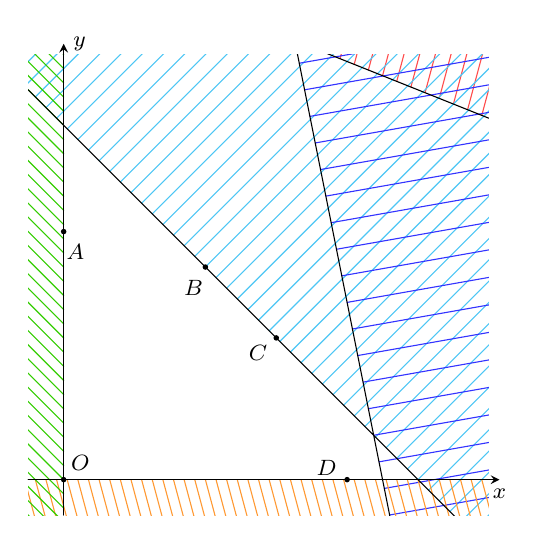
\begin{tikzpicture}[scale=1, font=\footnotesize, line join=round, line cap=round, >=stealth, x=0.45cm, y=0.45cm]
				\tikzset{declare function={f(\x)=15-0.4*(\x); g(\x)=10-\x; h(\x)=45-5*(\x);}}
				\def\xt{-1} \def\xp{12}
				\def\yd{-1} \def\yt{12}
				\begin{scope}
					\clip (\xt,\yd) rectangle (\xp,\yt);
					\foreach \i in {-3,-2.6,...,\xp} \draw[red!70!white] (\i,{f(\i)})--++(75:8);
					\foreach \j in {-2,-1.7,...,\xp} \draw[cyan!70!white] (\j,{g(\j)})--++(45:10);
					\foreach \k in {-1,-0.85,...,\xp} \draw[blue!80!white] (\k,{h(\k)})--++(10:8);
					\foreach \x in {-2,-1.7,...,\xp} \draw[orange!80!white] (\x,0)--++(-75:2);
					\foreach \y in {-2,-1.6,...,\yt} \draw[green!80!red] (0,\y)--++(135:2);
					\draw[domain=\xt:\xp] plot(\x,{f(\x)})
					plot(\x,{g(\x)})
					plot(\x,{h(\x)});
				\end{scope} 
				\draw[->] (\xt,0)--(\xp+0.3,0)node[below]{$x$};
				\draw[->] (0,\yd)--(0,\yt+0.3)node[right]{$y$};
				\foreach \p/\n/\g in {(0,0)/O/45, (0,7)/A/-60, (4,6)/B/-120, (6,4)/C/220, (8,0)/D/150} \fill \p node[shift={(\g:3mm)}]{$\n$} circle(1pt);
			\end{tikzpicture}
		\end{center}
		Miền nghiệm của hệ bất phương trình $(1)$ là ngũ giác $OABCD$ với $A(0;7)$; $O(0;0)$; $B(4;6)$, $C(6;4)$, $D(8;0)$. \\
		Vì giá trị lớn nhất của $f(x;y)=70x+90y$ đạt được tại đỉnh của miền nghiệm.\\
		Ta có $f(0;0)=0$, $f(0;7)=630$, $f(4;6)=600$, $f(6;4)=580$, $f(8;0)=560$.\\
		Suy ra $f(x;y)$ đạt giá trị lớn nhất tại $A(0;7)$.\\
		Vậy để đạt số điểm thưởng lớn nhất đội chơi cần pha chế $7$ lít nước loại B. 
	}
\end{ex}
\begin{ex}%[0D3V1-7]
	Một cửa hàng nhân dịp Tết đã đồng loạt giảm giá các sản phẩm. Trong đó có chương trình nếu mua một gói kẹo thứ hai trở đi sẽ được giảm $15\%$ so với giá ban đầu. Biết giá gói đầu là $80\,000$ đồng. Bạn An có $600\,000$ đồng. Hỏi bạn An có thể mua tối đa bao nhiêu gói kẹo?
	\shortans{$8$}
	\loigiai{
		Giả sử bạn An mua được $x$ gói kẹo ($x$ nguyên dương).\\
		Khi đó gói thứ nhất bạn An phải trả $80\,000$ đồng.\\
		Số gói kẹo còn lại là $x-1$ và bạn An chỉ phải trả
		\begin{center}
			$80\,000-15\% \cdot 80\,000 = 68\,000$ đồng (mỗi gói).
		\end{center}
		Vậy số tiền phải trả khi mua kẹo được tính theo công thức
		$$y=80\,000+(x-1)\cdot 68\,000=68\,000x+12\,000.$$
		Số tiền bạn An dùng mua kẹo phải không quá $600\,000$ đồng, suy ra
		$$68\,000x+12\,000 \le 600\,000 \Rightarrow x \le \dfrac{588\,000}{68\,000} \approx 8{,}588.$$
		Vậy với số tiền hiện có, bạn An chỉ có thể mua được tối đa $8$ gói kẹo.
	}
\end{ex}
\begin{ex}%[0H4V1-3]
	Cho $\tan \alpha=\dfrac{2}{5}$. Tính giá trị của biểu thức $A=\dfrac{4\sin \alpha + 3\cos \alpha}{5\sin \alpha - 2\cos \alpha}$ thu được kết quả dạng $-\dfrac{a}{b}$ với $\dfrac{a}{b}$ là phân số tối giản và $b\ne 0$. Tính $a+b$.
	\shortans{$19$}
	\loigiai{
		Vì $\tan \alpha=\dfrac{\sin \alpha}{\cos \alpha}=\dfrac{2}{5}$ nên $\cos \alpha \ne 0$.\\
		Chia cả tử và mẫu của $A$ cho $\cos \alpha$, ta được: 
		\[
		A=\dfrac{4 \dfrac{\sin \alpha}{\cos \alpha}+3}{5\dfrac{\sin \alpha}{\cos \alpha}-2}=\dfrac{4\tan \alpha+3}{5\tan \alpha-2}=\dfrac{4\cdot \dfrac{2}{5}+3}{5\cdot \dfrac{2}{5}-2}= \dfrac{\dfrac{8}{5}+3}{2-2}=\dfrac{\dfrac{8 + 15}{5}}{0}= \dfrac{23}{0}=-\dfrac{23}{5}.
		\]
		Vậy $a=23$, $b=5$ nên $a+b=28$.
	}
\end{ex}
\begin{ex}%[0H4V2-1]
	Từ vị trí $A$ người ta quan sát một cây cao.
	\begin{center}
		\usetikzlibrary{decorations.pathmorphing,shapes}
		\tikzset{
			treetop/.style = {
				decoration={random steps, segment length=0.4mm},
				decorate
			},
			trunk/.style = {
				decoration={random steps, segment length=2mm, amplitude=0.2mm},
				decorate
			}
		}
		\tikzset{
			man/.pic={%
				\fill [rounded corners=1.5] (0,0.4) -- (0,0.4 -- (0.4,0.5 -- (0.4,0.4) --
				(0.325,0.4) -- (0.325,0.7) -- (0.3,0.7) -- (0.3,0) -- (0.225,0) --
				(0.225,0.4) -- (0.175,0.4) -- (0.175,0) -- (0.1,0) -- (0.1,0.7) --
				(0.075,0.7) -- (0.075,0.4) -- cycle;
				\fill (0.2,0.9) circle (0.1);
				\coordinate (-head) at (0.2,1);
				\coordinate (-foot) at (0.2,0);
			}
		}
		\begin{tikzpicture}[scale=0.7, font=\footnotesize,line join = round, line cap = round, >=stealth]
			\path
			(-4,-2) coordinate (A)
			(0,1.2) coordinate (C)
			(0.2,-2.5) coordinate (T)
			(-4,-2.5) coordinate (H)
			(0,-2.5) coordinate (B)		
			;
			%\pic[red] at (-5.3,-2.5) (myman) {man};
			\foreach \w/\f in {0.3/30,0.2/50,0.1/70} {
				\fill [brown!\f!black, trunk] (0,0) ++(-\w/2,0) rectangle +(\w,-2.5);
			}
			\foreach \n/\f in {1.2/40,1/50,0.8/60,0.6/70,0.4/80} {
				\fill [green!\f!black, treetop] ellipse (\n/1.5 and \n);
			}
			\draw (H)--(T) (A)--(H) (A)--(C) (A)--(B);
			\pic[draw,"$40^{\circ}$", angle eccentricity=1.4,angle radius=0.8cm]{angle=B--A--C};
			\pic[draw,"$ $", angle eccentricity=1.4,angle radius=0.7cm]{angle=B--A--C};
			\draw pic[draw, angle radius=2mm]{right angle=B--H--A};
			\path (H)--(B) node[below,midway,sloped]{$15$ m};
			\foreach \x/\g in {A/180,B/-90,C/90,H/-90} \fill[black] (\x)+(\g:.3) node {$\x$};
		\end{tikzpicture}
	\end{center}
	Biết $AH=3$ (m), $HB=15$ (m), $\widehat{BAC}=40^\circ$. Khi đó chiều cao của cây là (tính chính xác đến hàng phần chục).
	\shortans{$12{,}7$}
	\loigiai{
		Vì tam giác $AHB$ vuông tại $H$ nên ta có $AB =\sqrt{AH^2+HB^2}= \sqrt{3^2+15^2}=\sqrt{9+225}=\sqrt{234}\approx 15{,}3$ m.\\
		Ta có \\
		$\sin \widehat{BAH}=\dfrac{BH}{AB}=\dfrac{15}{\sqrt{234}}\approx 0{,}984 \Rightarrow \widehat{BAH}\approx 78{,}6^\circ \Rightarrow \widehat{ABC} \approx 78{,}6^\circ \Rightarrow \widehat{ACB} \approx 61{,}4^\circ$.\\
		Áp dụng định lý sin cho tam giác $ABC$ ta có $\dfrac{BC}{\sin A}= \dfrac{AB}{\sin C}$.\\
		Suy ra $BC \approx 12{,}7$ m.
	}
\end{ex}
\begin{ex}%[0H4V3-2]
	\immini[thm]{Bác An cần đo khoảng cách từ một địa điểm $A$ trên bờ hồ đến một địa điểm $B$ ở giữa hồ. Bác sử dụng giác kế để chọn một điểm $C$ cùng nằm trên bờ với $A$ sao cho $\widehat{BAC}=45^\circ$, $\widehat{ACB}=85^\circ$ và $AC=60$\,m. Hỏi khoảng cách $AB$ bằng bao nhiêu mét (làm tròn kết quả đến hàng phần chục)?}{\begin{tikzpicture}[scale=1,font=\footnotesize,line cap=round,line join=round,>=stealth]
			\coordinate (A) at (0,0);
			\coordinate (C) at (4,0);
			\coordinate (B) at (4.5,3);
			\fill[cyan!30] (-.5,2) .. controls +(-70:2) and +(150:1) .. (2.5,1) .. controls +(-15:2) and +(-30:1) .. (5.5,3.5) .. controls +(150:1) and +(40:1) .. (3,4) .. controls +(-150:1.5) and +(100:2) .. cycle;
			\draw (A)--(B)--(C)--cycle;
			\foreach \d/\g in {A/-135, B/90, C/-45}
			\fill (\d) circle(1pt) node[shift={(\g:.3)}]{$\d$};
			\path pic[draw,angle radius=.3cm]{angle=C--A--B} (A) node[shift={(20:.8)}]{$ $} pic[draw,angle radius=.3cm]{angle=B--C--A} pic[draw,angle radius=.35cm]{angle=B--C--A} (C) node[shift={(150:.7)}]{$ $};
	\end{tikzpicture}}
	\shortans[]{$60{,}9$} 
	\loigiai{Xét tam giác $ABC$ có $\widehat{B}=180^\circ-\widehat{A}-\widehat{C}=50^\circ$.\\
		Áp dụng định lý sin trong tam giác $ABC$ ta được\[\dfrac{AB}{\sin C}=\dfrac{AC}{\sin B}\Rightarrow AB=\dfrac{AC\cdot\sin C}{\sin B}=\dfrac{60\cdot\sin85^\circ}{\sin50^\circ}\approx60{,}9 \text{(m)}.\]}
\end{ex}
\Closesolutionfile{ans}
\indapan{6}{ans/ans-CTST-0-OTGK1-De04-KQ}

